\documentclass{standalone}
\usepackage{tikz}
\usetikzlibrary{patterns, positioning}

\begin{document}
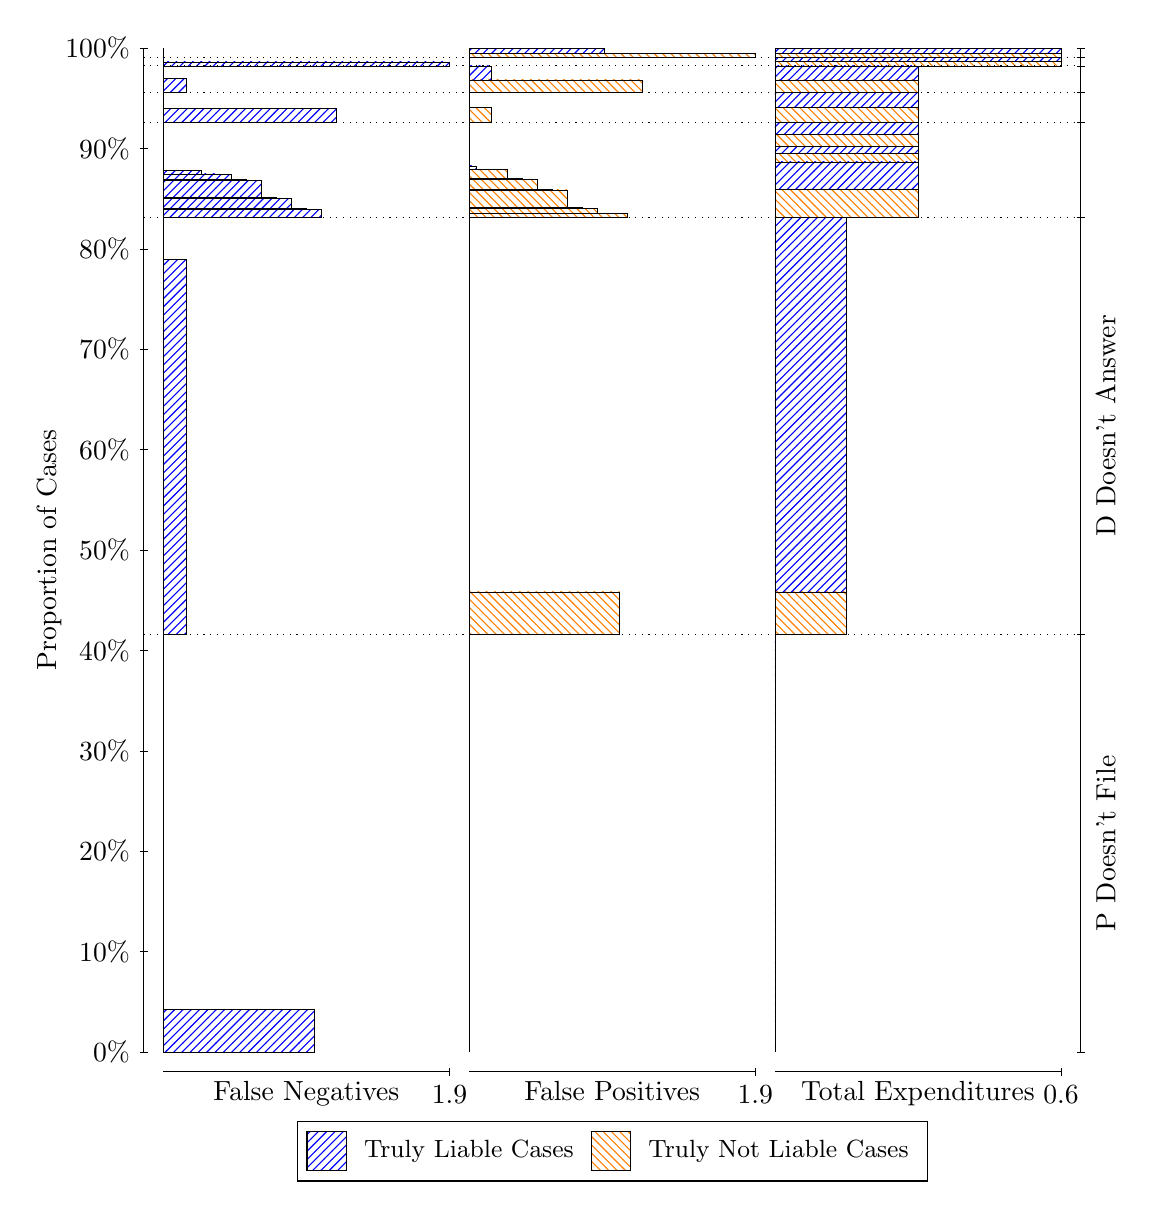
\begin{tikzpicture}
\draw[black, very thin] (1.5,1.75) -- (1.5,14.5);
\node[rotate=90, anchor=center] at (0.3, 8.125) {Proportion of Cases};
\draw[black, very thin] (1.45,1.75) -- (1.55,1.75);
\node[anchor=east] at (1.45, 1.75) {0\%};
\draw[black, very thin] (1.45,3.025) -- (1.55,3.025);
\node[anchor=east] at (1.45, 3.025) {10\%};
\draw[black, very thin] (1.45,4.3) -- (1.55,4.3);
\node[anchor=east] at (1.45, 4.3) {20\%};
\draw[black, very thin] (1.45,5.575) -- (1.55,5.575);
\node[anchor=east] at (1.45, 5.575) {30\%};
\draw[black, very thin] (1.45,6.85) -- (1.55,6.85);
\node[anchor=east] at (1.45, 6.85) {40\%};
\draw[black, very thin] (1.45,8.125) -- (1.55,8.125);
\node[anchor=east] at (1.45, 8.125) {50\%};
\draw[black, very thin] (1.45,9.4) -- (1.55,9.4);
\node[anchor=east] at (1.45, 9.4) {60\%};
\draw[black, very thin] (1.45,10.675) -- (1.55,10.675);
\node[anchor=east] at (1.45, 10.675) {70\%};
\draw[black, very thin] (1.45,11.95) -- (1.55,11.95);
\node[anchor=east] at (1.45, 11.95) {80\%};
\draw[black, very thin] (1.45,13.225) -- (1.55,13.225);
\node[anchor=east] at (1.45, 13.225) {90\%};
\draw[black, very thin] (1.45,14.5) -- (1.55,14.5);
\node[anchor=east] at (1.45, 14.5) {100\%};

\draw[black, very thin] (13.4,1.75) -- (13.4,14.5);
\draw[black, very thin] (13.35,1.75) -- (13.45,1.75);
\node[anchor=west] at (13.35, 1.75) {};
\draw[black, very thin] (13.35,7.0516) -- (13.45,7.0516);
\node[anchor=west] at (13.35, 7.0516) {};
\draw[black, very thin] (13.35,12.352) -- (13.45,12.352);
\node[anchor=west] at (13.35, 12.352) {};
\draw[black, very thin] (13.35,13.553) -- (13.45,13.553);
\node[anchor=west] at (13.35, 13.553) {};
\draw[black, very thin] (13.35,13.932) -- (13.45,13.932);
\node[anchor=west] at (13.35, 13.932) {};
\draw[black, very thin] (13.35,14.274) -- (13.45,14.274);
\node[anchor=west] at (13.35, 14.274) {};
\draw[black, very thin] (13.35,14.385) -- (13.45,14.385);
\node[anchor=west] at (13.35, 14.385) {};
\draw[black, very thin] (13.35,14.5) -- (13.45,14.5);
\node[anchor=west] at (13.35, 14.5) {};

\draw[black, very thin, pattern color=blue, pattern=north east lines] (1.75,1.75) rectangle (3.6623,2.2912);
\draw[black, very thin, pattern color=orange, pattern=north west lines] (1.75,2.2912) rectangle (1.75,7.0516);
\draw[black, very thin, pattern color=blue, pattern=north east lines] (1.75,7.0516) rectangle (2.0368,11.811);
\draw[black, very thin, pattern color=orange, pattern=north west lines] (1.75,11.811) rectangle (1.75,12.352);
\draw[black, very thin, pattern color=blue, pattern=north east lines] (1.75,12.352) rectangle (3.7579,12.448);
\draw[black, very thin, pattern color=blue, pattern=north east lines] (1.75,12.448) rectangle (3.5667,12.463);
\draw[black, very thin, pattern color=blue, pattern=north east lines] (1.75,12.463) rectangle (3.3754,12.587);
\draw[black, very thin, pattern color=blue, pattern=north east lines] (1.75,12.587) rectangle (3.1842,12.599);
\draw[black, very thin, pattern color=blue, pattern=north east lines] (1.75,12.599) rectangle (2.993,12.816);
\draw[black, very thin, pattern color=blue, pattern=north east lines] (1.75,12.816) rectangle (2.8018,12.83);
\draw[black, very thin, pattern color=blue, pattern=north east lines] (1.75,12.83) rectangle (2.6105,12.893);
\draw[black, very thin, pattern color=blue, pattern=north east lines] (1.75,12.893) rectangle (2.4193,12.902);
\draw[black, very thin, pattern color=blue, pattern=north east lines] (1.75,12.902) rectangle (2.2281,12.95);
\draw[black, very thin, pattern color=orange, pattern=north west lines] (1.75,12.95) rectangle (1.75,13.553);
\draw[black, very thin, pattern color=blue, pattern=north east lines] (1.75,13.553) rectangle (3.9491,13.734);
\draw[black, very thin, pattern color=orange, pattern=north west lines] (1.75,13.734) rectangle (1.75,13.932);
\draw[black, very thin, pattern color=blue, pattern=north east lines] (1.75,13.932) rectangle (2.0368,14.112);
\draw[black, very thin, pattern color=orange, pattern=north west lines] (1.75,14.112) rectangle (1.75,14.274);
\draw[black, very thin, pattern color=blue, pattern=north east lines] (1.75,14.274) rectangle (5.3833,14.325);
\draw[black, very thin, pattern color=orange, pattern=north west lines] (1.75,14.325) rectangle (1.75,14.385);
\draw[black, very thin, pattern color=orange, pattern=north west lines] (1.75,14.385) rectangle (1.75,14.436);
\draw[black, very thin, pattern color=blue, pattern=north east lines] (1.75,14.436) rectangle (1.75,14.5);
\draw[black, very thin, pattern color=orange, pattern=north west lines] (5.6333,1.75) rectangle (5.6333,6.5104);
\draw[black, very thin, pattern color=blue, pattern=north east lines] (5.6333,6.5104) rectangle (5.6333,7.0516);
\draw[black, very thin, pattern color=orange, pattern=north west lines] (5.6333,7.0516) rectangle (7.5456,7.5922);
\draw[black, very thin, pattern color=blue, pattern=north east lines] (5.6333,7.5922) rectangle (5.6333,12.352);
\draw[black, very thin, pattern color=orange, pattern=north west lines] (5.6333,12.352) rectangle (7.6412,12.396);
\draw[black, very thin, pattern color=orange, pattern=north west lines] (5.6333,12.396) rectangle (7.45,12.404);
\draw[black, very thin, pattern color=orange, pattern=north west lines] (5.6333,12.404) rectangle (7.2588,12.467);
\draw[black, very thin, pattern color=orange, pattern=north west lines] (5.6333,12.467) rectangle (7.0675,12.481);
\draw[black, very thin, pattern color=orange, pattern=north west lines] (5.6333,12.481) rectangle (6.8763,12.698);
\draw[black, very thin, pattern color=orange, pattern=north west lines] (5.6333,12.698) rectangle (6.6851,12.7);
\draw[black, very thin, pattern color=orange, pattern=north west lines] (5.6333,12.7) rectangle (6.6851,12.709);
\draw[black, very thin, pattern color=orange, pattern=north west lines] (5.6333,12.709) rectangle (6.4939,12.834);
\draw[black, very thin, pattern color=orange, pattern=north west lines] (5.6333,12.834) rectangle (6.3026,12.849);
\draw[black, very thin, pattern color=orange, pattern=north west lines] (5.6333,12.849) rectangle (6.1114,12.955);
\draw[black, very thin, pattern color=blue, pattern=north east lines] (5.6333,12.955) rectangle (5.7289,13.003);
\draw[black, very thin, pattern color=blue, pattern=north east lines] (5.6333,13.003) rectangle (5.6333,13.553);
\draw[black, very thin, pattern color=orange, pattern=north west lines] (5.6333,13.553) rectangle (5.9202,13.751);
\draw[black, very thin, pattern color=blue, pattern=north east lines] (5.6333,13.751) rectangle (5.6333,13.932);
\draw[black, very thin, pattern color=orange, pattern=north west lines] (5.6333,13.932) rectangle (7.8325,14.094);
\draw[black, very thin, pattern color=blue, pattern=north east lines] (5.6333,14.094) rectangle (5.9202,14.274);
\draw[black, very thin, pattern color=orange, pattern=north west lines] (5.6333,14.274) rectangle (5.6333,14.334);
\draw[black, very thin, pattern color=blue, pattern=north east lines] (5.6333,14.334) rectangle (5.6333,14.385);
\draw[black, very thin, pattern color=orange, pattern=north west lines] (5.6333,14.385) rectangle (9.2667,14.436);
\draw[black, very thin, pattern color=blue, pattern=north east lines] (5.6333,14.436) rectangle (7.3544,14.5);
\draw[black, very thin, pattern color=orange, pattern=north west lines] (9.5167,1.75) rectangle (9.5167,6.5104);
\draw[black, very thin, pattern color=blue, pattern=north east lines] (9.5167,6.5104) rectangle (9.5167,7.0516);
\draw[black, very thin, pattern color=orange, pattern=north west lines] (9.5167,7.0516) rectangle (10.425,7.5922);
\draw[black, very thin, pattern color=blue, pattern=north east lines] (9.5167,7.5922) rectangle (10.425,12.352);
\draw[black, very thin, pattern color=orange, pattern=north west lines] (9.5167,12.352) rectangle (11.333,12.7);
\draw[black, very thin, pattern color=blue, pattern=north east lines] (9.5167,12.7) rectangle (11.333,13.054);
\draw[black, very thin, pattern color=orange, pattern=north west lines] (9.5167,13.054) rectangle (11.333,13.159);
\draw[black, very thin, pattern color=blue, pattern=north east lines] (9.5167,13.159) rectangle (11.333,13.255);
\draw[black, very thin, pattern color=orange, pattern=north west lines] (9.5167,13.255) rectangle (11.333,13.405);
\draw[black, very thin, pattern color=blue, pattern=north east lines] (9.5167,13.405) rectangle (11.333,13.553);
\draw[black, very thin, pattern color=orange, pattern=north west lines] (9.5167,13.553) rectangle (11.333,13.751);
\draw[black, very thin, pattern color=blue, pattern=north east lines] (9.5167,13.751) rectangle (11.333,13.932);
\draw[black, very thin, pattern color=orange, pattern=north west lines] (9.5167,13.932) rectangle (11.333,14.094);
\draw[black, very thin, pattern color=blue, pattern=north east lines] (9.5167,14.094) rectangle (11.333,14.274);
\draw[black, very thin, pattern color=orange, pattern=north west lines] (9.5167,14.274) rectangle (13.15,14.334);
\draw[black, very thin, pattern color=blue, pattern=north east lines] (9.5167,14.334) rectangle (13.15,14.385);
\draw[black, very thin, pattern color=orange, pattern=north west lines] (9.5167,14.385) rectangle (13.15,14.436);
\draw[black, very thin, pattern color=blue, pattern=north east lines] (9.5167,14.436) rectangle (13.15,14.5);
\draw[black, dotted] (1.5,7.0516) -- (13.4,7.0516);
\draw[black, dotted] (1.5,12.352) -- (13.4,12.352);
\draw[black, dotted] (1.5,13.553) -- (13.4,13.553);
\draw[black, dotted] (1.5,13.932) -- (13.4,13.932);
\draw[black, dotted] (1.5,14.274) -- (13.4,14.274);
\draw[black, dotted] (1.5,14.385) -- (13.4,14.385);
\draw[black, very thin] (1.75,1.5) -- (5.3833,1.5);
\node[anchor=north] at (3.5667, 1.5) {False Negatives};
\draw[black, very thin] (5.3833,1.45) -- (5.3833,1.55);
\node[anchor=north] at (5.3833, 1.45) {1.9};

\draw[black, very thin] (5.6333,1.5) -- (9.2667,1.5);
\node[anchor=north] at (7.45, 1.5) {False Positives};
\draw[black, very thin] (9.2667,1.45) -- (9.2667,1.55);
\node[anchor=north] at (9.2667, 1.45) {1.9};

\draw[black, very thin] (9.5167,1.5) -- (13.15,1.5);
\node[anchor=north] at (11.333, 1.5) {Total Expenditures};
\draw[black, very thin] (13.15,1.45) -- (13.15,1.55);
\node[anchor=north] at (13.15, 1.45) {0.6};

\node[black, centered, rotate=90] at (13.72, 4.4008) {P Doesn't File};
\node[black, centered, rotate=90] at (13.72, 9.7018) {D Doesn't Answer};






\draw (7.449999999999999,1.5) node[draw=none] (baseCoordinate) {};
\begin{scope}[align=center]
        \matrix[scale=0.5, draw=black, below=0.5cm of baseCoordinate, nodes={draw}, column sep=0.1cm]{
            \node[rectangle, draw, minimum width=0.5cm, minimum height=0.5cm, pattern=north east lines, pattern color=blue] {}; &
            \node[draw=none, font=\small] (B) {Truly Liable Cases}; &
            \node[rectangle, draw, minimum width=0.5cm, minimum height=0.5cm, pattern=north west lines, pattern color=orange] {}; &
            \node[draw=none, font=\small] (B) {Truly Not Liable Cases}; \\
            };
\end{scope}

\end{tikzpicture}
\end{document}